\begin{figure*}[t]
\centering
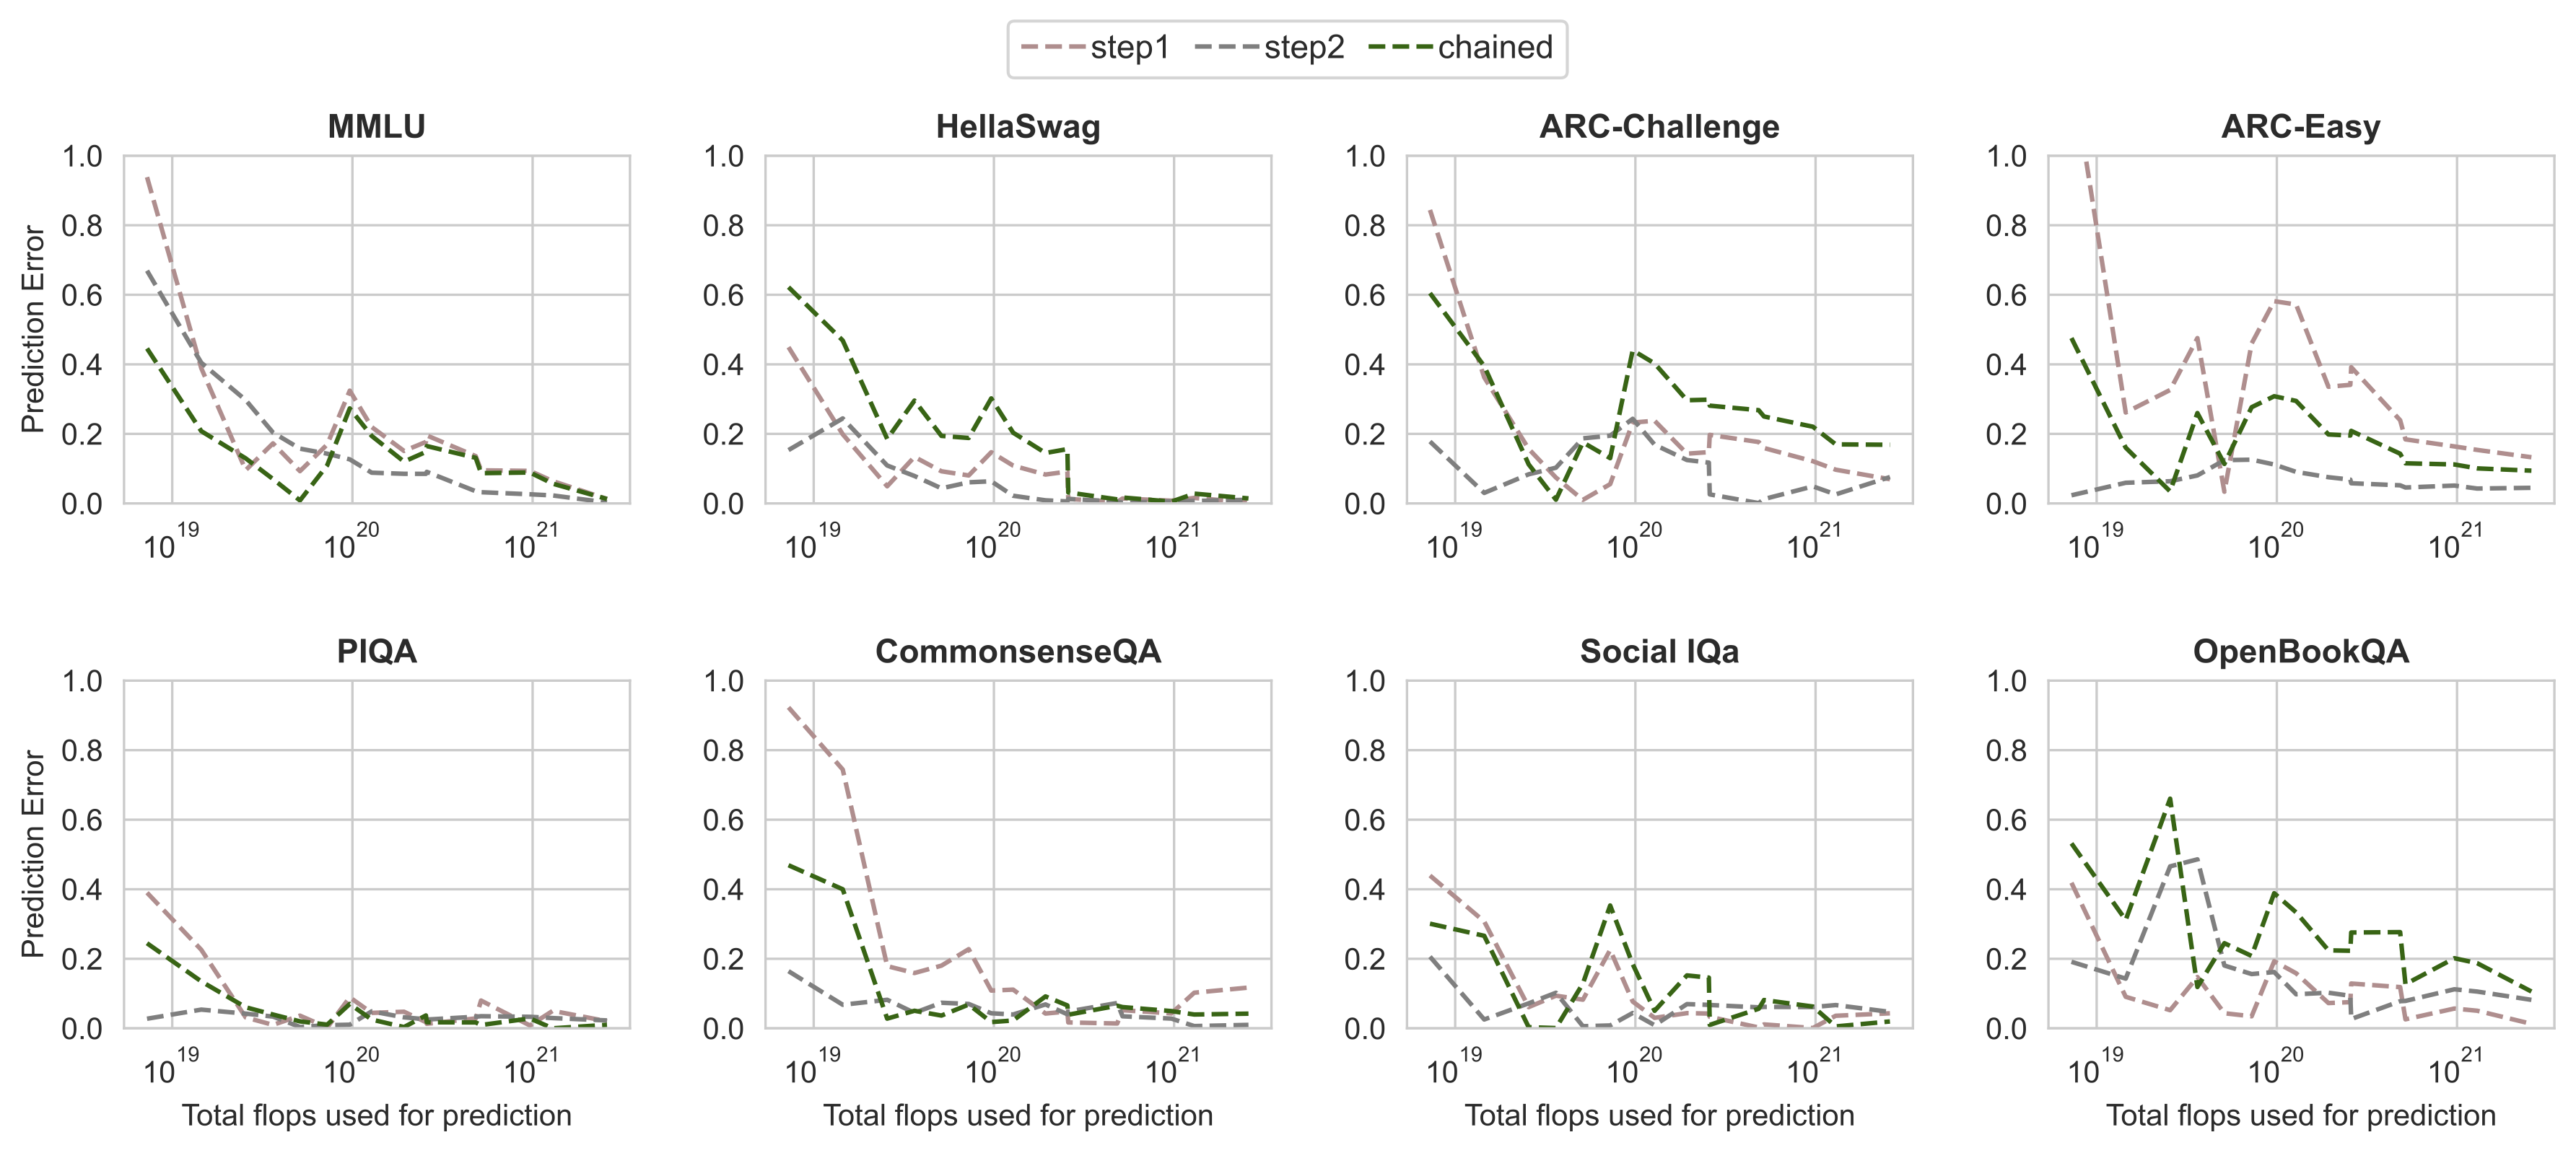
\includegraphics[width=0.8\linewidth]{images/compute_vs_error/vary_flops_error_all.png}
\vspace{-12pt}
\caption{
    Prediction error on the 7B-4T target model as a function of the total compute-FLOPs used in the ladder models for prediction. The left-most point uses only the smallest model (190M-1xC) for prediction. The right-most point uses the full ladder (all 16 models). The prediction error generally reduces as the ladder FLOPs increase. ARC-C, ARC-E, and OBQA display higher variation (which can be attributed to the variation analysis in \S\ref{sec_variance_analysis}), but still have a downward trend.
}
\label{fig:compute_vs_error_flops}
\vspace{-8pt}
\end{figure*}
